\documentclass[12pt,a4paper]{report}
\usepackage[a4paper,left=1.5in,right=1.0in,top=1.0in,bottom=1.0in]{geometry}
\usepackage{graphicx}
\usepackage{float}

\usepackage{listings}
\usepackage{xcolor}
\usepackage{caption}

\lstset{
  breaklines=true,
  basicstyle=\ttfamily\footnotesize,
  frame=single,
  columns=fullflexible,
  keepspaces=true,
  tabsize=2,
  commentstyle=\color{gray},
  keywordstyle=\color{blue},
  stringstyle=\color{orange},
  showstringspaces=false
}



\renewcommand{\baselinestretch}{1.25}
\setlength{\parindent}{2em}
\setlength{\parskip}{.75 cm}
\usepackage{mathptmx}
\usepackage{xcolor}
\usepackage{listings}
\usepackage{url}
\usepackage{tabto}
\usepackage{hyperref}
\usepackage[format=plain,
            labelfont={bf,it},
            textfont=it]{caption}


\begin{document}
 \begin{titlepage}
  \begin{center}
   \begin{LARGE}
    \textbf{REAL-TIME CHAT APPLICATION}\\[.75cm]
   \end{LARGE}
   \textbf{\large A}\\
   \textbf{\large Industrial Oriented Mini Project Report}\\[.5cm]  
   \textit{\large Submitted in partial fulfillment of the requirements for the award of the degree of}\\[1.5cm]
   \textup{\Large \textbf{Bachelor of Technology}}\\
   \textbf{\Large in}\\
   \textup{\Large \textbf{Computer Science and Engineering}}\\[1cm]
   \textup{\large Submitted by}\\[1cm]
   \begin{table}[ht]
    \centering
    \begin{tabular}{l r}
     {\large E.Arjun} & {\large 22SS1A0512}\\
     {\large N.Mahesh} & {\large 22SS1A0531}\\
     {\large R.Prabhas} & {\large 22SS1A0541}\\
     {\large S.Srinivas} & {\large 22SS1A0548}\\
     
    \end{tabular}
   \end{table}
   \textup{\Large Under the guidance of}\\[.5cm]
   \textbf{\Large Dr.G.Priyanka Jeeva Karunya}\\[.5cm]
   \textup{\Large Assistant Professor}\\[.5cm]
   % COLLEGE LOGO
   \begin{figure}[h!]
    \centering 
    \includegraphics[width= 4cm \linewidth]{jntuhlogo.png}
       \label{fig:enter-label}
   \end{figure}
   \textup{\Large Department of Computer Science and Engineering}\\[.5cm]
   \textup{\Large JNTUH University College of Engineering Sultanpur}\\[.25cm] 
   \textup{\large Sultanpur(V), Pulkal(M), Sangareddy district, Telangana-502273}\\[.25cm] 
   \textup{\Large June 2025}\\[.5cm]\end{center}
 \end{titlepage}



\pagenumbering{arabic}
\addcontentsline{toc}{chapter}{Certificate}

\begin{center}
 {\large\textbf{JNTUH UNIVERSITY COLLEGE OF ENGINEERING SULTANPUR}}\\
 \textup{\normalsize{Sultanpur(V), Pulkal(M), Sangareddy-502273, Telangana}}\\[1cm]
 
 \begin{figure}[h!]
  \centering
  \includegraphics[width=4cm\linewidth]{jntuhlogo.png}
 \end{figure}
 
 {\large\textup{Department of Computer Science and Engineering}}\\[1.0cm]
 {\Large \textbf{\textit{Certificate}}}\\
 \vspace{0.5cm}
\end{center}
This is to certify that the Industrial Oriented Mini Project Report work entitled “\textbf{REAL-TIME CHAT APPLICATION}”  is a bonafide work carried out by a team consisting of \textbf{E.Arjun} bearing Roll no. \textbf{22SS1A0512},  \textbf{N.Mahesh} bearing Roll no. \textbf{22SS1A0531}, \ \textbf{R.Prabhas} bearing Roll no. \textbf{22SS1A0541}, textbf{S.Srinivas} bearing Roll no. \textbf{22SS1A0548} in partial fulfillment of the requirements for the degree of BACHELOR OF TECHNOLOGY in COMPUTER SCIENCE AND ENGINEERING discipline to  Jawaharlal Nehru Technological University Hyderabad Unviersity College of Engineering Sultanpur during the academic year 2024 - 2025.\\ \\
The results embodied in this report have not been submitted to any other University or Institution for the award of any degree or diploma.\\
\vspace{1cm}\\
\textbf{Guide \hfill Head of the Department\\}
\textbf{Dr.G.Priyanka Jeeva Karunya\hfill Dr. G. Narasimha\\}
\textbf{Assistant Professor \hfill Professor \& Principal\\ }
\begin{center}
 \vspace{0.5 cm}
 %\vspace{1.5cm}
\end{center}

\begin{center}
\textbf{External Examiner}
\end{center}




\newpage
\addcontentsline{toc}{chapter}{Declaration} 
\begin{center}
{\LARGE \textbf{\textit{Declaration}}}
\end{center} 
\vspace{2cm}
{\large We hereby declare that the Research Project entitled “\textbf{REAL-TIME CHAT APPLICATION}” is a bonafide work carried out by a team consisting of \textbf {E.Arjun} bearing Roll no. \textbf{22SS1A0512},  \textbf{N.Mahesh} bearing Roll no. \textbf{22SS1A0531},  \textbf{R.Prabhas} bearing Roll no. \textbf{22SS1A0541},
\textbf{S.Srinivas} bearing Roll no. \textbf{22SS1A0548} in partial fulfillment of the requirements for the degree of Bachelor of Technology in Computer Science and Engineering discipline to  Jawaharlal Nehru Technological University Hyderabad University College of Engineering Sultanpur during the academic year 2023- 2024. The results embodied in this report have not been submitted to any other University or Institution for the award of any degree or diploma.}\\ \\
\vspace{4.0cm}
\begin{table}[ht]
 \begin{flushright}
  \begin{tabular}{l r}
  {\large E.Arjun} & {\large 22SS1A0512}\\
  {\large N.Mahesh} & {\large 22SS1A0531}\\
  {\large R.Prabhas} & {\large 22SS1A0541}\\
   {\large S.Srinivas} & {\large 22SS1A0548}\\
  
 \end{tabular}
 \end{flushright}
\end{table}


\newpage
\addcontentsline{toc}{chapter}{Acnowledgement} 
\begin{center}
{\LARGE \textbf{\textit{Acknowledgment}}}
\end{center}
\vspace{1cm}
{\large {We wish to take this opportunity to express our deep gratitude to all those who helped us in various ways during our Research Project report work. It is our pleasure to acknowledge the help of all those individuals who were responsible for foreseeing the successful completion of our Project report.\\
\hspace*{35pt}We express our sincere gratitude to \textbf{\large Dr. G Narsimha, Professor and Principal}, JNTUHUCES for his support during the course period.\\ \\
\hspace*{35pt}We sincerely thank \textbf{\large Dr. Y .Raghavender Rao, Professor and Vice Principal}, JNTUHCES for his kind help and co-operation.\\

\hspace*{35pt}We are thankful to out guide \textbf{\large Dr.G.Priyanka Jeeva Karunya  Assistant Professor} for her constant support, effective suggestions throughout the course period.\\\\
\hspace*{35pt}Finally,we express our gratitude with great admiration and respect to our faculty for their moral support and encouragement throughout the course.}}
\vspace{4.0cm}
\begin{table}[ht]
 \begin{flushright}
  \begin{tabular}{l r}
  {\large E.Arjun} & {\large 22SS1A0512}\\
  {\large N.Mahesh} & {\large 22SS1A0531}\\
  {\large R.Prabhas} & {\large 22SS1A0541}\\
  {\large S.Srinivas} & {\large 22SS1A0548}\\
  
 \end{tabular}
 \end{flushright}
\end{table}
%\vspace{1.0cm}



\newpage
%\renewcommand{\baselinestretch}{0.1}
\tableofcontents
\addtocontents{toc}

\newpage
\addcontentsline{toc}{chapter}{Abstract}
\begin{LARGE}{\textbf{\textit{\Huge \hspace{35pt} \hspace{35pt}  \hspace{35pt}Abstract}}}
\vspace{1.0cm}
{\Large 

{\large In the modern era of instant communication, this project focuses on developing a real-
time chat application inspired by WhatsApp, utilizing the MERN stack (MongoDB, 
Express.js, React.js, Node.js) and Socket.io for real-time messaging. The primary goal is 
to create a highly responsive and interactive messaging platform that ensures seamless 
instant messaging, real-time notifications, and message status updates, including sent, 
delivered, and read receipts.
Unlike traditional chat applications, this system leverages Socket.io for bi-directional 
communication, ensuring efficient real-time event handling between the client and server. 
The MERN stack provides a flexible and scalable architecture:
- MongoDB serves as the NoSQL database for storing user data, chat histories, and media 
files.
- Express.js acts as the backend framework, handling API requests and server-side logic.
- React.js powers the frontend, offering an interactive and user-friendly experience.
- Node.js serves as the runtime environment, enabling seamless integration between the 
frontend and backend.
The system aims to replicate core WhatsApp functionalities, including one-on-one chats, 
message notifications, and real-time delivery status tracking. Future enhancements may 
introduce group chats, media sharing, user authentication, and end-to-end encryption, 
ensuring security and reliability.
 
{\large 

}}
\end{LARGE}
\vspace{4.0cm}
\begin{table}[ht]
 \begin{flushright}
  \begin{tabular}{l r}
  
 \end{tabular}
 \end{flushright}
\end{table}

\newpage
\addcontentsline{toc}{chapter}{List of figures}
\listoffigures
 
\newpage
\pagenumbering{arabic}
\chapter{INTRODUCTION}

This project is a mobile-friendly, real-time messaging web application inspired by WhatsApp Web. It is developed using the MERN stack (MongoDB, Express.js, React.js, and Node.js), with WebSockets (via Socket.IO) to enable seamless bi-directional communication between clients. Unlike the traditional WhatsApp system that relies on phone numbers, this application introduces a modern and secure authentication system based on email, powered by JSON Web Tokens (JWT), cookies, and email verification using NodeMailer and Brevo SMTP services.

The application supports essential messaging features such as 1-to-1 real-time text and image communication, friend request management (by email or username), user profile editing, and status posting similar to WhatsApp’s “Status” feature. It features a user-friendly React-based UI that mirrors WhatsApp Web, while ensuring responsiveness and interactivity through modern libraries such as React Icons, React Hot Toast, and React Router.

This full-stack system serves as an academic mini project, designed not only to demonstrate real-time chat capabilities but also to integrate user session management, secure authentication flows, and modern frontend UI/UX techniques. The project is highly modular, scalable, and designed with clean architecture in mind, making it a foundational prototype for more complex messaging applications.

\section{Project Overview}
This project aims to replicate WhatsApp Web’s core functionality, including email-based registration, verification, and secure login. It leverages the MERN stack to offer dynamic routing, a real-time chat engine via WebSocket connections, and seamless image/media transmission through Cloudinary integration. The system supports sending and receiving friend requests using either username or registered email. Once accepted, users can initiate conversations or view the status of their contacts. With Socket.IO, messages are delivered in real-time without requiring manual page refreshes, offering a responsive and interactive messaging experience.

\section{Problem Statement}
Many real-time messaging platforms in the market, including WhatsApp, Telegram, and Messenger, are proprietary, phone-number-dependent, and often unsuitable for academic or personal customization. These platforms do not allow insight into internal architecture or extensibility for learning purposes. There exists a need for a simple, secure, and modular real-time communication system built using widely-used open-source technologies.

This project addresses the gap by developing a customizable, open-source alternative that provides secure email-based login and verification, WebSocket-based real-time messaging, profile management, and an intuitive UI. It not only mimics the functionality of WhatsApp Web but is also a flexible base for educational, experimental, and scalable real-world use cases.

\section{Purpose}
The purpose of this project is to build a secure, browser-based, WhatsApp-inspired communication system using modern full-stack technologies. By avoiding phone-based login and instead using email and JWT for authentication, the project showcases a more adaptable and widely applicable login flow. Real-time messaging, file/image sharing, friend request handling, and status posting are supported, making the application both practical and comprehensive.

This project is designed to help developers understand how different pieces of a full-stack system interact — from frontend user events, to backend API handling, real-time sockets, database models, and middleware authentication. It encourages students to move beyond theory and apply best practices in real-time system design, asynchronous operations, state management, and secure backend logic.

\section{Existing System}
Current systems like WhatsApp, Telegram, and Messenger are robust and feature-rich, but they are closed-source, which restricts learning, experimentation, and customization. They rely heavily on phone-based authentication and mobile-first design. For learners and developers aiming to understand or prototype messaging systems, these platforms do not offer transparency or adaptability.

Moreover, most commercial messaging platforms are optimized for large-scale use cases and may involve complex integrations like end-to-end encryption, voice-over-IP, and proprietary protocols, which are difficult to replicate or learn from in smaller academic projects. Therefore, there is a need for a transparent, simplified, and open alternative that is also scalable and secure.

\section{Literature Survey}
\begin{itemize}
    \item \textbf{Real-time Communication:} WebSockets (via Socket.IO) enable two-way persistent connections ideal for real-time systems. Literature confirms their effectiveness over HTTP polling for instant messaging.
    
    \item \textbf{Authentication and Authorization:} JSON Web Tokens (JWT) combined with HTTP-only cookies ensure secure, stateless authentication suitable for single-page applications.
    
    \item \textbf{Email Verification Systems:} NodeMailer with Brevo SMTP provides a reliable and programmable way to send OTPs and verify users during registration, improving application trustworthiness and preventing spam.
    
    \item \textbf{Frontend UI/UX Design:} Clean, WhatsApp-like UI built using React and utility libraries (React Icons, Hot Toast) is proven to enhance user engagement and familiarity.
    
    \item \textbf{Friend Management:} Social systems often benefit from mutual acceptance models (requests and approvals), which can be handled efficiently through NoSQL relationships in MongoDB.
\end{itemize}

\section{Conclusion}
The ChatApp project delivers a functional, real-time messaging platform that integrates both frontend and backend technologies effectively. It solves the problem of limited accessibility and customization in proprietary platforms by offering an open, modular, and email-based solution for chatting and media exchange. The project provides valuable learning in full-stack development, authentication, session management, WebSocket handling, and deployment readiness.

With scope for future features like group chat, end-to-end encryption, and video/voice calling, this project lays a solid foundation for building scalable, real-time applications in both academic and startup ecosystems.



\newpage
\chapter{SYSTEM ANALYSIS}

\section{Data Collection}
Data collection in this project involves gathering and managing user inputs and messages in real-time to enable seamless communication. It includes storing and handling user credentials, chat histories, and message metadata.

\begin{itemize}
    \item User registration details such as email, username, and password are collected for authentication purposes.
    \item Chat messages are transmitted instantly and stored temporarily for session continuity.
    \item Metadata such as timestamps and message statuses (sent, delivered, read) are recorded.
    \item Media files (images) can be uploaded and stored as part of message data.
\end{itemize}

\section{Reliability}
\begin{itemize}
    \item The project ensures reliable message delivery by using Socket.io, which maintains a persistent connection for instant communication, reducing message loss even during network fluctuations.
    \item User authentication is securely handled using JWT and cookies to prevent unauthorized access, ensuring only valid users can send and receive messages. This protects user data and maintains system integrity.
    \item Error handling mechanisms are implemented to detect and resolve connection or server issues promptly, preventing app crashes and maintaining continuous operation.
    \item The system stores message metadata to confirm delivery status, providing users with reliable feedback on their communications, thereby building trust in the application’s functionality.
\end{itemize}

\section{Availability}
\begin{itemize}
    \item The application is designed to be accessible 24/7, allowing users to send and receive messages at any time without downtime, which is essential for real-time communication.
    \item Session persistence enables users to remain logged in across visits, providing seamless access without repeated logins, thus enhancing availability by reducing user friction.
    \item The system architecture supports quick recovery from server interruptions, ensuring minimal downtime. Automatic reconnection mechanisms help maintain user connectivity.
    \item Hosting the backend on reliable platforms or local servers ensures consistent uptime. Regular monitoring and maintenance help prevent unexpected outages.
\end{itemize}

\section{Portability}
\begin{itemize}
    \item \textbf{Cross-Platform Compatibility:}  The project is developed using the MERN stack (MongoDB, Express.js, React.js, Node.js), making it accessible on various devices and browsers without the need for installation. Users can chat seamlessly from desktops, tablets, or smartphones.
    \item \textbf{Easy Deployment:} Using Node.js backend and standard web technologies enables deployment on multiple platforms, including cloud servers, local machines, or hosting services. This flexibility supports diverse hosting environments.
    \item \textbf{Minimal External Dependencies:} Reliance mainly on standard libraries and Socket.io reduces compatibility issues across different environments, enhancing portability by avoiding heavy or platform-specific dependencies.
\end{itemize}

Overall, by leveraging these characteristics, this chat application ensures smooth operation across multiple devices and browsers. Its lightweight, modular design allows easy deployment and adaptation to various platforms, making it highly portable and accessible to a wide range of users.

\section{Performance}
\begin{itemize}
\item The use of Node.js in the MERN stack enables fast, non-blocking server-side processing, supporting multiple simultaneous user connections efficiently for smooth real-time messaging.
\item Socket.io optimizes data transfer by maintaining persistent WebSocket connections, reducing latency compared to traditional HTTP requests, which results in quicker message delivery.
\item The React.js frontend ensures dynamic and responsive user interfaces, improving load times and overall application responsiveness across devices.
\item Asynchronous operations within the MERN architecture prevent UI freezing during message sending and receiving, enhancing interaction speed and ensuring a seamless chat experience.
\item Efficient management of message data with MongoDB and minimal server overhead contribute to stable performance, even as the number of active users grows. Scalability can be further enhanced with future optimizations.
\end{itemize}

\section{Conclusion}
This chat application developed using the MERN stack demonstrates effective integration of modern web technologies to deliver a real-time, user-friendly messaging platform.

The system ensures reliable data collection and secure authentication using JWT and cookies, while real-time communication is achieved through Socket.io. The MERN stack’s full-stack capabilities allow seamless handling of both client-side and server-side processes.

Portability is enhanced by leveraging React.js for a cross-platform frontend, and Node.js with Express.js for a robust backend API. MongoDB offers flexible and scalable data storage for user and message information.

Performance is optimized through asynchronous communication and persistent WebSocket connections, delivering a smooth and responsive chat experience. Overall, this project lays a strong foundation for future enhancements like group chats, media sharing, and encryption.

\newpage

\newpage



\chapter{EXISTING SYSTEM}

This chapter provides an in-depth review of current messaging systems and communication platforms that inspired this project. Understanding the existing solutions helps highlight their strengths and limitations, and clarifies the unique contributions and improvements proposed by this Chat App.

\section{Overview of Popular Messaging Platforms}

Popular applications such as WhatsApp, Telegram, Facebook Messenger, Signal, and WeChat dominate the instant messaging landscape. These platforms provide a rich set of features including text messaging, multimedia sharing, voice and video calls, end-to-end encryption, group chats, and status updates. They serve millions to billions of users globally, ensuring high availability, robust security, and seamless user experience.

Most of these platforms are mobile-first and rely heavily on phone number-based authentication for identity verification and contact discovery. Their backends are typically highly optimized and distributed to manage enormous loads and ensure real-time delivery of messages, even under varying network conditions.

\section{Authentication and User Identification}

Phone number-based authentication is widely adopted in existing messaging apps due to its simplicity and integration with device telephony. It enables automatic contact synchronization by matching phone numbers with users' contact lists. However, this method has limitations — users without mobile phones or those preferring alternative identification methods cannot easily register or log in.

Some platforms, like Telegram and Facebook Messenger, also allow email or username-based login but are exceptions rather than the norm. The dependency on phone numbers raises privacy concerns for some users, and phone number recycling can cause security issues in rare cases.

\section{Real-Time Communication Technologies}

To deliver instant messaging, these platforms implement a variety of technologies. Early systems used HTTP polling or long-polling, which were resource-intensive and inefficient. Modern applications have shifted to WebSocket protocols, enabling persistent bi-directional connections between client and server.

WebSocket technology provides low latency and reduces overhead, improving message delivery speed and user experience. For example, WhatsApp Web uses a combination of WebSocket and proprietary protocols to maintain session synchronization and deliver real-time updates seamlessly.

\section{Limitations and Challenges}

Despite their success, existing platforms have some drawbacks:

\begin{itemize}
    \item \textbf{Closed-source nature:} Most leading messaging apps are proprietary, making it impossible for developers or students to examine, learn, or extend their internal workings.
    \item \textbf{Phone number dependency:} The reliance on mobile numbers excludes users who prefer email or other login methods, limiting accessibility and flexibility.
    \item \textbf{Complexity and feature bloat:} The vast array of features may overwhelm users seeking simpler communication tools or developers needing clean, focused systems.
    \item \textbf{Lack of educational tools:} There is a shortage of open-source, well-documented projects that combine real-time messaging, secure authentication, and rich user interactions in a single package for learning purposes.
\end{itemize}

\section{Gaps Addressed by This Project}

This project targets these gaps by providing:

\begin{itemize}
    \item A fully open, modular codebase developed with widely-used web technologies (MERN stack).
    \item Email-based authentication with JWT and cookie management, avoiding phone number limitations.
    \item Real-time, one-to-one messaging using Socket.IO for WebSocket communication.
    \item Features like friend request handling, status posting, and profile editing to replicate core social interactions.
    \item A clean, WhatsApp-like UI built with React, focusing on simplicity and responsiveness.
\end{itemize}

By addressing these areas, this project offers a valuable learning resource for developers and a foundation for customizable real-time communication systems suitable for both academic and practical applications.



\newpage

\newpage




\chapter{REQUIREMENT SPECIFICATION}

This chapter outlines the hardware and software requirements necessary for developing, deploying, and running the MERN-based real-time chat application effectively.

\section{Hardware Requirements}
\begin{itemize}
    \item \textbf{Processor:} Intel i5 or higher for smooth development and testing of real-time features.
    \item \textbf{RAM:} Minimum 8 GB (Recommended: 16 GB) to handle simultaneous backend, frontend, and database services.
    \item \textbf{Hard Disk:} At least 100 GB of free space to accommodate databases, media files, and development dependencies.
    \item \textbf{Display:} 1366x768 resolution or higher for proper UI/UX testing and responsive design.
    \item \textbf{Internet Connectivity:} Required for real-time testing, npm installations, and using SMTP/email verification services.
\end{itemize}

\section{Software Requirements}
\begin{itemize}
    \item \textbf{Operating System:} Windows 10/11, Linux (Ubuntu preferred), or macOS.
    \item \textbf{IDE/Code Editor:} Visual Studio Code for writing, debugging, and managing frontend/backend code.
    \item \textbf{Browser:} Latest versions of Google Chrome or Firefox for testing and debugging the React frontend.
    \item \textbf{API Testing Tool:} Postman for testing Express.js REST APIs.
    \item \textbf{Version Control:} Git and GitHub for source code management and collaboration.
\end{itemize}

\section{Development Stack}
\begin{itemize}
    \item \textbf{Frontend:} React.js (with React Router DOM, React Icons, React Hot Toast).
    \item \textbf{Backend:} Node.js and Express.js.
    \item \textbf{Database:} MongoDB for storing user data, chat history, and media metadata.
    \item \textbf{Real-Time Communication:} Socket.io for persistent two-way communication.
    \item \textbf{Authentication:} JWT (JSON Web Tokens) and cookies for secure login and protected routes.
\end{itemize}

\section{Third-Party Services and Libraries}
\begin{itemize}
    \item \textbf{Nodemailer:} For sending email-based OTP verification links.
    \item \textbf{Bravao SMTP Service:} Used as the SMTP server provider for email delivery.
    \item \textbf{Cloudinary:} For uploading and retrieving media files like images.
    \item \textbf{bcryptjs:} For securely hashing user passwords.
    \item \textbf{CORS \& Cookie-Parser:} For managing cross-origin requests and session cookies.
\end{itemize}

\section{Functional Requirements}
\begin{itemize}
    \item \textbf{User Registration \& Login:} Secure user onboarding using email, password, and email verification.
    \item \textbf{One-to-One Chat:} Real-time text and image messaging.
    \item \textbf{Friend Requests:} Ability to send/accept requests via email or username.
    \item \textbf{Status Feature:} Users can update and view their status.
    \item \textbf{Profile Editing:} Users can update their profile info including display picture, username, and bio.
\end{itemize}

\section{Non-Functional Requirements}
\begin{itemize}
    \item \textbf{Scalability:} Modular architecture to support future additions like group chats or encryption.
    \item \textbf{Security:} Encrypted passwords, protected routes, and secure data transfer.
    \item \textbf{Performance:} Low-latency communication via WebSockets.
    \item \textbf{Usability:} Clean UI/UX similar to WhatsApp Web for easy navigation.
    \item \textbf{Maintainability:} Code organized with reusable components and middleware.
\end{itemize}


\newpage



\chapter{TECHNOLOGIES USED}


\begin{figure}[H]
    \centering
    \includegraphics[width=12cm]{Tech Used.png}
    \caption{Status Page Showing Secure Login State}
\end{figure}



This chapter outlines the various technologies, frameworks, and services used in the development of the MERN stack-based Chat App. The choice of each technology reflects its suitability for creating scalable, real-time, and user-friendly chat applications.

\section{MongoDB}
\begin{itemize}
    \item MongoDB is a NoSQL, document-oriented database used for storing user data, chat messages, and media metadata in JSON-like format.
    \item It allows for dynamic schema designs, making it highly flexible for handling different types of chat data.
    \item Mongoose is used as an Object Data Modeling (ODM) library to define schemas and interact with MongoDB more easily.
    \item Collections are used to store user profiles, chat histories, message status, and friend requests.
    \item MongoDB supports horizontal scaling, making it efficient as user data grows in future implementations.
\end{itemize}

\section{Express.js}
\begin{itemize}
    \item Express.js is a minimalist Node.js web application framework used for handling backend routes and REST APIs.
    \item It simplifies the server-side logic for user authentication, message routing, and file uploads.
    \item Middleware such as cookie-parser, cors, and dotenv are integrated to handle sessions, cross-origin requests, and secure environment configurations.
    \item The backend APIs follow RESTful architecture principles for better scalability and maintenance.
    \item Express is also responsible for integrating Socket.io and connecting frontend users to WebSocket endpoints.
\end{itemize}

\section{React.js}
\begin{itemize}
    \item React.js is used to build the frontend user interface, offering a component-based architecture and reactive rendering.
    \item React Router DOM helps manage multiple routes such as login, signup, chat, and profile pages in a single-page application (SPA).
    \item React Hot Toast is used to give real-time user notifications like “Message sent,” “Login successful,” etc.
    \item React Icons provide ready-to-use icons that closely resemble WhatsApp UI elements like send, chat, call, and emoji.
    \item The virtual DOM enables efficient updates without reloading the page, providing a seamless chat experience.
\end{itemize}

\section{Node.js}
\begin{itemize}
    \item Node.js serves as the backend runtime environment, enabling the use of JavaScript for server-side development.
    \item It is non-blocking and event-driven, making it ideal for real-time applications where multiple users are connected simultaneously.
    \item It supports asynchronous processing using Promises and async/await for efficient API request handling.
    \item With built-in modules and package support via npm, Node.js allows quick integration of external libraries.
    \item It is used to run both the Express server and the Socket.io WebSocket server for real-time message exchange.
\end{itemize}

\section{Socket.io}
\begin{itemize}
    \item Socket.io is a JavaScript library that enables bi-directional, real-time communication between client and server using WebSockets.
    \item It provides a persistent connection between users, allowing instant delivery of messages without needing to refresh the page.
    \item Events such as ‘message’, ‘typing’, ‘user-connected’, and ‘user-disconnected’ are handled efficiently.
    \item Socket.io handles automatic reconnection and fallback for poor network conditions, improving reliability.
    \item It is fully integrated with Express and React for seamless real-time communication.
\end{itemize}

\section{Supporting Technologies and Services}
\begin{itemize}
    \item \textbf{JWT (jsonwebtoken):} Used for secure user authentication and route protection.
    \item \textbf{bcryptjs:} Hashes user passwords for secure storage.
    \item \textbf{Cloudinary:} Cloud-based service for storing and retrieving profile pictures and media messages.
    \item \textbf{Nodemailer with Bravao SMTP:} Sends email verification and OTPs to users during signup or password reset.
    \item \textbf{VS Code:} Main code editor used for writing, debugging, and managing frontend and backend code.
    \item \textbf{Postman:} Used for testing backend API endpoints during development.
\end{itemize}


\newpage


\chapter{ARCHITECTURE}

The architecture of the ChatApp is based on the MERN stack (MongoDB, Express.js, React.js, Node.js), combined with real-time communication using Socket.io. This architecture ensures scalability, responsiveness, and high performance. It follows a modular client-server model with support for RESTful APIs and WebSocket connections.



\begin{figure}[H]
    \centering
    \includegraphics[width=15cm]{big.png}
    \caption{Architecture Diagram}
    \caption*{This diagram represents the overall architecture of the ChatApp, including the client-side React app, Node.js server, database (MongoDB), and WebSocket communication using Socket.io.}
\end{figure}


\begin{figure}[H]
    \centering
    \includegraphics[width=12cm]{ClassDiagram.png}
    \caption{Class Diagram}
    \caption*{The class diagram illustrates the structure of the main backend entities such as User, Message, Chat, and how they relate to one another in the system's object model.}
\end{figure}


\begin{figure}[H]
    \centering
    \includegraphics[width=12cm]{Use case diagram.png}
    \caption{Use Case Diagram}
    \caption*{This diagram depicts the major use cases from the user's perspective, including registration, login, sending messages, uploading media, and managing sessions.}
\end{figure}





\begin{figure}[H]
    \centering
    \includegraphics[width=12cm]{sequence-digram.png}
    \caption{Sequence Diagram}
    \caption*{The sequence diagram represents the sequence of interactions between components during the login and messaging process — from user action to server response.}
\end{figure}



\begin{figure}[H]
    \centering
    \includegraphics[width=11cm]{state diagram.png}
    \caption{State Diagram}
    \caption*{The state diagram shows different states a user session can be in — such as Logged Out, OTP Pending, Logged In, and Chatting — along with transitions between those states.}
\end{figure}

\begin{figure}[H]
    \centering
    \includegraphics[width=11cm]{deployment diagram.png}
    \caption{Deployment Diagram}
    \caption*{The deployment diagram outlines the physical deployment of software artifacts, showing how the client app, backend server, and database are hosted and interact.}
\end{figure}



\section{System Design Overview}
\begin{itemize}
    \item The system consists of three primary layers: the frontend (React), the backend server (Node.js with Express), and the database (MongoDB).
    \item A WebSocket connection using Socket.io allows real-time communication between users through the server.
    \item API endpoints are used for user registration, login, media upload, and data retrieval.
    \item Cloud services like Cloudinary are used for image storage, while email services like Bravao SMTP handle OTP-based email verification.
\end{itemize}

\section{Client-Side Architecture}
\begin{itemize}
    \item The frontend is built using React.js and is structured into modular components like ChatWindow, MessageInput, ContactList, etc.
    \item React Router DOM is used to handle navigation between pages like login, signup, profile, and chat.
    \item Axios is used to send HTTP requests to the backend server for user authentication, profile updates, and chat history retrieval.
    \item State management is achieved using React Hooks (useState, useEffect, useContext), which help in managing user data, online status, and live messages.
    \item WebSocket events are emitted and received via the Socket.io client to enable instant messaging.
\end{itemize}

\section{Server-Side Architecture}
\begin{itemize}
    \item Node.js with Express.js is used to handle backend logic, authentication, database operations, and Socket.io events.
    \item Express middleware such as cors, cookie-parser, and dotenv handle CORS policies, cookies, and environment configurations.
    \item Authentication is managed using JWTs, ensuring secure access to protected routes like chat and profile.
    \item RESTful APIs support CRUD operations for users, messages, and file uploads.
    \item Socket.io is integrated to manage real-time message transmission, online status, and typing indicators.
\end{itemize}

\section{Database Architecture}


\begin{itemize}
    \item MongoDB stores all persistent data, including user credentials, chat histories, and media metadata.
    \item Collections include:
    \begin{itemize}
        \item \textbf{Users:} Stores user profiles, hashed passwords, online/offline status.
        \item \textbf{Messages:} Stores chat messages, sender/receiver IDs, timestamps, delivery/read status.
        \item \textbf{Media:} Stores metadata for uploaded files such as URLs, file types, and timestamps.
    \end{itemize}
    \item Mongoose schemas are used to define models and perform validation.
    \item References (ObjectIds) are used to link messages to users for efficient queries.
\end{itemize}

\section{Socket.io Event Flow}
\begin{itemize}
    \item \textbf{Connection:} A new socket connection is initialized when the user logs in.
    \item \textbf{Message Events:} The server listens for 'send-message' and emits 'receive-message' to the appropriate recipient in real-time.
    \item \textbf{Typing Indicators:} Emits 'typing' and 'stop-typing' events to notify other users.
    \item \textbf{Disconnection:} When a user logs out or disconnects, the socket is terminated, and the user's status is updated.
    \item \textbf{Broadcasting:} Socket.io rooms are used to send messages to specific user pairs, enabling one-to-one messaging without leaks.
\end{itemize}

\section{Deployment and Hosting Architecture}
\begin{itemize}
    \item The application can be deployed on cloud platforms like Render, Vercel, or Heroku.
    \item The backend (Express + Socket.io) and frontend (React) are deployed separately and communicate through environment-configured URLs.
    \item Static frontend files are built using `npm run build` and hosted via Vercel or Netlify.
    \item MongoDB Atlas provides managed database hosting and ensures high availability.
    \item The system uses environment variables (.env) to manage sensitive information such as database URIs and JWT secrets.
\end{itemize}

\newpage


\chapter{ FILE STRUCTURE}

This chapter provides the file structure overview of both the backend and frontend of the ChatApp. The project follows a modular and scalable architecture using the MERN stack. The backend is built with Node.js and Express.js, while the frontend uses React.js. Socket.io is used for real-time messaging, and MongoDB serves as the database.

\section{Backend File Structure}

\begin{verbatim}
�� server/
│
├── .env
├── .gitignore
├── index.js
├── package.json
├── package-lock.json
│
├── �� config/
│   ├── cloudinary.js
│   ├── db.js
│   ├── InsertDataInDB.js
│   ├── jwtToken.js
│   ├── nodeMailer.js
│   └── socket.io.js
│
├── �� controllers/
│   ├── auth.controller.js
│   ├── message.controller.js
│   └── user.controller.js
│
├── �� middlewares/
│   ├── auth.middleware.js
│   └── authSockert.middleware.js
│
├── �� models/
│   ├── chat.model.js
│   ├── FriendRequest.model.js
│   ├── message.model.js
│   ├── status.model.js
│   ├── statusvideo.model.js
│   └── user.model.js
│
├── �� routes/
│   ├── auth.route.js
│   ├── message.route.js
│   └── user.route.js
│
└── �� utils/
    ├── mailTemplate.js
    └── verifyOtpTemp.js
\end{verbatim}

\newpage

\section{Frontend File Structure}

\begin{verbatim}
�� frontend/
│
├── package.json
├── package-lock.json
├── README.md
├── .gitignore
│
├── �� public/
│   ├── index.html
│   ├── favicon.ico
│   ├── manifest.json
│   ├── robots.txt
│   └── (images: login.png, logout.png, etc.)
│
├── �� src/
│   ├── index.js
│   ├── App.js
│   ├── App.css, index.css, css.css
│   ├── socket.js
│   ├── reportWebVitals.js
│   ├── setupTests.js
│   ├── logo.svg
│
│   ├── �� lib/
│   │   └── axios.js
│
│   ├── �� pages/
│   │   ├── HomePage.jsx
│   │   ├── SignupPage.jsx
│   │   ├── EditProfilePage.jsx
│   │   ├── ProfilePage.jsx, ProfilePage.css
│   │   ├── SettingsPage.jsx
│   │   ├── verifyOtpPage.jsx
│   │   └── OtpVerificationPage.css
│
│   ├── �� components/
│       ├── �� HomePage/
│       │   ├── contextDef.jsx
│       │   ├── Left.jsx, Middle.jsx, Right.jsx
│       │
│       │   ├── �� LeftComponents/
│       │   │   └── Icons.jsx, Icons.css
│       │
│       │   ├── �� MiddleComponents/
│       │   │   ├── AddFriends.jsx, AIChat.jsx, Channels.jsx
│       │   │   ├── Chats.jsx, Community.jsx, Notifications.jsx
│       │   │   ├── Profile.jsx, Settings.jsx, Status.jsx
│       │   │   ├── SettingsOption.jsx
│       │   │
│       │   │   └── �� SubMiddle/
│       │   │       ├── MyStatus.jsx, StatusVideo.jsx, User.jsx
│
│       │   ├── �� RightComponents/
│       │   │   ├── ChatBubble.jsx, MessagePart.jsx
│       │   │   ├── RightPart.jsx, RightPartCard.jsx
│       │   │   ├── RAddFriends.jsx, RAiChat.jsx
│       │   │   ├── RChannels.jsx, RCommunity.jsx
│       │   │   ├── RNotifications.jsx, RProfilePart.jsx
│       │   │   ├── RSettings.jsx, RStatus.jsx
│       │   │
│       │   │   └── �� SubRight/
│       │   │       ├── AddFriendRight.jsx, CmtyChnl.jsx
│       │   │       ├── NotificationProfile.jsx
│       │   │       ├── StatusViewer.jsx, TypingDots.jsx
│
│       ├── �� SignUpLoginPage/
│       │   └── SignUpLogin.jsx
│
│       └── �� utils/
│           ├── BtnLoader.jsx
│           └── Loader.jsx
\end{verbatim}

\newpage


\chapter{CODE}
\section{App.js}
Below is the complete React code for the main `App.js` component.

\begin{lstlisting}[language=JavaScript, caption=React App Component, label={lst:appjs}, breaklines=true, breakatwhitespace=true, basicstyle=\ttfamily\footnotesize, frame=single]
import React, { useContext, useEffect } from "react";
import './App.css';
import { BrowserRouter } from 'react-router-dom';
import { Navigate, Route, Routes } from "react-router-dom";
import SignupPage from "./pages/SignupPage";
import HomePage from "./pages/HomePage";
import ProfilePage from "./pages/ProfilePage";
import Settings from "./components/HomePage/MiddleComponents/Settings";
import { Toaster } from 'react-hot-toast';
import { ContextDef } from "./components/HomePage/contextDef";
import Spinner from "./components/utils/Loader";
import OtpVerificationPage from "./pages/verifyOtpPage";

const App = () => {
  const { authUser, checkAuth, isCheckingAuth} = useContext(ContextDef);

  useEffect(() => {
    checkAuth();  // Call checkAuth to validate user on mount
  }, [checkAuth]);

  if (isCheckingAuth && !authUser) {
    return (
      <Spinner/>
    );
  }

  return (
    <>
      <style>
        {`
          @keyframes spin {
            0% { transform: rotate(0deg); }
            100% { transform: rotate(360deg); }
          }
        `}
      </style>

      <BrowserRouter>
        <Routes>
          <Route path="/" element={authUser ? (authUser?.isVerified ? (<Navigate to="/home" />) : <Navigate to="/verify" />) : <Navigate to="/signup" />} />
          <Route path="/signup" element={<SignupPage />} />
          <Route path="/home" element={authUser ? (authUser?.isVerified ? (<HomePage />) : <Navigate to="/verify" />) : <Navigate to="/signup" />} />
          <Route path="/profile" element={authUser ? (authUser?.isVerified ? (<ProfilePage />) : <Navigate to="/verify" />) : <Navigate to="/signup" />} />
          <Route path="/settings" element={authUser ? (authUser?.isVerified ? (<Settings />) : <Navigate to="/verify" />) : <Navigate to="/signup" />} />
          <Route path="/verify" element={authUser ? (authUser?.isVerified ? (<Navigate to="/home" />) : <OtpVerificationPage />) : <Navigate to="/signup" />} />
        </Routes>
      </BrowserRouter>
      <Toaster />
    </>
  );
};

export default App;
\end{lstlisting}


\section{SignUpLogin.js}

Below is the complete React code for the `SignUpLogin.js` component which handles both sign-up and login functionalities.

\lstset{
  language=JavaScript,
  caption=SignUpLogin Component,
  label={lst:signuplogin},
  breaklines=true,
  breakatwhitespace=true,
  basicstyle=\ttfamily\footnotesize,
  frame=single,
  columns=fullflexible,
  keepspaces=true
}

\begin{lstlisting}
import React, { useContext, useState } from 'react';
import axios from 'axios';
import './SignUpLogin.css';
import { useNavigate } from 'react-router-dom';
import toast from 'react-hot-toast';
import { axiosInstance } from '../../lib/axios';
import { ContextDef } from '../HomePage/contextDef';
import BtnLoader from '../utils/BtnLoader';

function SignUpLogin() {
  const navigate = useNavigate();
  const { login, signup, isLoggingIn, isSigningUp } = useContext(ContextDef);

  const [signUpUser, setSignUpUser] = useState({
    name: '',
    email: '',
    password: '',
  });

  const [loginUser, setLoginUser] = useState({
    email: '',
    password: '',
  });

  const [errorMessage, setErrorMessage] = useState('');

  const handleSignUpSubmit = async (e) => {
    e.preventDefault();
    try {
      const move = await signup(signUpUser);
      if (move) navigate('/home');
    } catch (error) {
      setErrorMessage(error.response?.data?.message || 'Something went wrong');
    }
  };

  const handleLoginSubmit = async (e) => {
    e.preventDefault();
    try {
      const move = await login(loginUser);
      if (move) navigate('/home');
    } catch (error) {
      setErrorMessage(error.response?.data?.message || 'Something went wrong');
    }
  };

  return (
    <>
      <div className="SignUpLogin">
        <input type="checkbox" id="flip" />

        <div className="cover">
          <div className="front info-container">
            <h1 id="info-title">Join Us!</h1>
            <p id="info-message">
              Sign up to create an account and explore our features.
            </p>
          </div>
          <div className="back info-container">
            <h1 id="info-title">Welcome Back!</h1>
            <p id="info-message">
              To stay connected, please login with your personal information.
            </p>
          </div>
        </div>

        {/* Sign-Up Form */}
        <div className="wrapper">
          <form onSubmit={handleSignUpSubmit}>
            <h2>Sign Up</h2>
            <div className="input-field">
              <input
                type="text"
                onChange={(e) =>
                  setSignUpUser({ ...signUpUser, name: e.target.value })
                }
                required
              />
              <label>Enter your name</label>
            </div>
            <div className="input-field">
              <input
                type="email"
                onChange={(e) =>
                  setSignUpUser({ ...signUpUser, email: e.target.value })
                }
                required
              />
              <label>Enter your email</label>
            </div>
            <div className="input-field">
              <input
                type="password"
                onChange={(e) =>
                  setSignUpUser({ ...signUpUser, password: e.target.value })
                }
                required
              />
              <label>Enter your password</label>
            </div>
            <button type="submit" style={{
              display: 'flex', justifyContent: 'center', alignItems: 'center',
            }}>
              {isSigningUp ? (<BtnLoader />) : "Register"}
            </button>
            <div className="register">
              <p>
                Have an account?
                <label className="orange" htmlFor="flip">
                  Login now
                </label>
              </p>
            </div>
          </form>
        </div>

        {/* Login Form */}
        <div className="wrapper">
          <form onSubmit={handleLoginSubmit}>
            <h2>Login</h2>
            <div className="input-field">
              <input
                type="email"
                onChange={(e) =>
                  setLoginUser({ ...loginUser, email: e.target.value })
                }
                required
              />
              <label>Enter your email</label>
            </div>
            <div className="input-field">
              <input
                type="password"
                onChange={(e) =>
                  setLoginUser({ ...loginUser, password: e.target.value })
                }
                required
              />
              <label>Enter your password</label>
            </div>
            <div className="forget">
              <label htmlFor="remember">
                <input type="checkbox" id="remember" />
                <p>Remember me</p>
              </label>
              <a href="#">Forgot password?</a>
            </div>
            <button type="submit" style={{
              display: 'flex', justifyContent: 'center', alignItems: 'center',
            }}>
              {isLoggingIn ? (<BtnLoader />) : "Log In"}
            </button>
            <div className="register">
              <p>
                Don't have an account?
                <label className="orange" htmlFor="flip">
                  Sign Up now
                </label>
              </p>
            </div>
          </form>
        </div>
      </div>

      {errorMessage && <div className="error-message">{errorMessage}</div>}
    </>
  );
}

export default SignUpLogin;
\end{lstlisting}


\section{HomePage.js}

This section contains the `HomePage` component, which displays a three-part layout using the `Left`, `Middle`, and `Right` components with a full-screen flex container.

\lstset{
  language=JavaScript,
  caption=HomePage Component,
  label={lst:homepage},
  breaklines=true,
  breakatwhitespace=true,
  basicstyle=\ttfamily\footnotesize,
  frame=single,
  columns=fullflexible,
  keepspaces=true
}

\begin{lstlisting}
import React from 'react';
import Left from '../components/HomePage/Left';
import Middle from '../components/HomePage/Middle';
import Right from '../components/HomePage/Right';

function HomePage() {
  const fullAppStyle = {
    height: '100dvh',
    width: '100dvw',
    position: 'fixed',
    top: '0',
    left: '0',
    display: 'flex',
    flexDirection: 'row',
    justifyContent: 'center',
    alignItems: 'center',
    backgroundColor: 'yellow',
  };

  return (
    <div style={fullAppStyle}>
      <Left />
      <Middle />
      <Right />
    </div>
  );
}

export default HomePage;
\end{lstlisting}


\section{ProfilePage.js}

The `ProfilePage` component allows users to view and update their profile picture, name, email, and account details. It also handles image uploads using `FileReader` and updates the profile via context.

\lstset{
  language=JavaScript,
  caption=ProfilePage Component,
  label={lst:profilepage},
  breaklines=true,
  breakatwhitespace=true,
  basicstyle=\ttfamily\footnotesize,
  frame=single,
  columns=fullflexible,
  keepspaces=true
}

\begin{lstlisting}
import { useContext, useState } from "react";

import { FaCamera, FaUser } from "react-icons/fa";
import { MdEmail } from "react-icons/md";

import "./ProfilePage.css";
import { ContextDef } from "../components/HomePage/contextDef";

const ProfilePage = () => {
  const { authUser, isUpdatingProfile, updateProfile } = useContext(ContextDef);
  const [selectedImg, setSelectedImg] = useState(null);

  const handleImageUpload = async (e) => {
    const file = e.target.files[0];
    if (!file) return;

    const reader = new FileReader();
    reader.readAsDataURL(file);

    reader.onload = async () => {
      const base64Image = reader.result;
      setSelectedImg(base64Image);
      await updateProfile({ profilePic: base64Image });
    };
  };

  return (
    <div className="profile-page">
      <div className="profile-container">
        <div className="profile-card">
          <div className="profile-header">
            <h1 className="profile-title">Profile</h1>
            <p className="profile-subtitle">Your profile information</p>
          </div>

          <div className="profile-avatar-section">
            <div className="profile-avatar-wrapper">
              <img
                src={selectedImg || authUser.profilePic || "/avatar.png"}
                alt="Profile"
                className="profile-avatar"
              />
              <label
                htmlFor="avatar-upload"
                className={
                  \`avatar-upload-btn ${isUpdatingProfile ? "uploading" : ""}\`
                }
              >
                <FaCamera className="camera-icon" />
                <input
                  type="file"
                  id="avatar-upload"
                  className="hidden"
                  accept="image/*"
                  onChange={handleImageUpload}
                  disabled={isUpdatingProfile}
                />
              </label>
            </div>
            <p className="avatar-helper-text">
              {isUpdatingProfile ? "Uploading..." : "Click the camera icon to update your photo"}
            </p>
          </div>

          <div className="profile-info">
            <div className="info-group">
              <div className="info-label">
                <FaUser className="info-icon" />
                Full Name
              </div>
              <p className="info-data">{authUser?.name}</p>
            </div>

            <div className="info-group">
              <div className="info-label">
                <MdEmail className="info-icon" />
                Email Address
              </div>
              <p className="info-data">{authUser?.email}</p>
            </div>
          </div>

          <div className="account-info">
            <h2 className="account-title">Account Information</h2>
            <div className="account-details">
              <div className="account-row">
                <span>Member Since</span>
                <span>{authUser.createdAt?.split("T")[0]}</span>
              </div>
              <div className="account-row no-border">
                <span>Account Status</span>
                <span className="active-status">Active</span>
              </div>
            </div>
          </div>
        </div>
      </div>
    </div>
  );
};

export default ProfilePage;
\end{lstlisting}


\section{Settings.js}

The `Settings` component displays the user’s profile along with a list of configurable settings. It includes a logout button that logs the user out and redirects to the sign-up page.

\lstset{
  language=JavaScript,
  caption=Settings Component,
  label={lst:settings},
  breaklines=true,
  breakatwhitespace=true,
  basicstyle=\ttfamily\footnotesize,
  frame=single,
  columns=fullflexible,
  keepspaces=true
}

\begin{lstlisting}
import React, { useContext } from 'react';
import './Settings.css';
import SettingsOption from './SettingsOption';

import { MdLogout } from "react-icons/md";
import { FaKey, FaLock, FaComments, FaBell, FaKeyboard, FaQuestionCircle } from 'react-icons/fa';
import { ContextDef } from '../contextDef';
import { useNavigate } from 'react-router-dom';

const Settings = () => {
  const { authUser, logout } = useContext(ContextDef);
  const navigate = useNavigate();

  const logoutSubmit = async (e) => {
    try {
      await logout();
      navigate('/signup');
    } catch (error) {
      console.log('Something went wrong');
    }
  };

  return (
    <div className="settings-container">
      <div className="settings-header">
        <h2>Settings</h2>
        <input type="text" placeholder="Search settings" className="search-input" />
      </div>

      <div className="profile-section">
        <img src={authUser?.profilePic || "/avatar.png"} alt="Profile" className="profile-pic" />
        <div className="settings-profile-info">
          <h3>{authUser?.name || "Mahesh"}</h3>
          <p>{authUser?.status || "Better to call, Instead text"}</p>
        </div>
      </div>

      <div className="options-list">
        <SettingsOption icon={<FaKey />} title="Account" description="Security notifications, account info" />
        <SettingsOption icon={<FaLock />} title="Privacy" description="Blocked contacts, disappearing messages" />
        <SettingsOption icon={<FaComments />} title="Chats" description="Theme, wallpaper, chat settings" />
        <SettingsOption icon={<FaBell />} title="Notifications" description="Message notifications" />
        <SettingsOption icon={<FaKeyboard />} title="Keyboard shortcuts" description="Quick actions" />
        <SettingsOption icon={<FaQuestionCircle />} title="Help" description="Help center, contact us, privacy policy" />
      </div>

      <div className="log-out-container">
        <button onClick={logoutSubmit} className="logout-class">
          <div className="logout-icon"><MdLogout /></div>
          <div className="logout-btn">Log out</div>
        </button>
      </div>
    </div>
  );
};

export default Settings;
\end{lstlisting}


\section{OTPVerificationPage.jsx}

The following is the complete implementation of the \texttt{OTPVerificationPage.js} component. It handles sending and verifying OTPs for email verification in the React application. It uses React hooks like \texttt{useState}, \texttt{useContext}, and \texttt{useNavigate}, and relies on context for backend interaction.

\lstset{
  language=JavaScript,
  caption=OTPVerificationPage Component,
  label={lst:otpverification},
  breaklines=true,
  breakatwhitespace=true,
  basicstyle=\ttfamily\footnotesize,
  frame=single,
  columns=fullflexible,
  keepspaces=true
}

\begin{lstlisting}
import { useContext, useState } from "react";
import { MdVerified } from "react-icons/md";
import "./OtpVerificationPage.css";
import { ContextDef } from "../components/HomePage/contextDef";
import { useNavigate } from "react-router-dom";
import { FaUser } from "react-icons/fa";
import { MdEmail } from "react-icons/md";
import { FaHouseUser } from "react-icons/fa6";

const OTPVerificationPage = () => {
  const [otp, setOtp] = useState("");
  const [isVerified, setIsVerified] = useState(false);
  const [otpSent, setOtpSent] = useState(false);

  const { authUser, sendVerifyOtpFun, verifyEmail } = useContext(ContextDef);
  const navigate = useNavigate();

  const handleSendOtp = async () => {
    try {
      const move = await sendVerifyOtpFun();
      setOtpSent(move);
    } catch (error) {
      console.log(error.response?.data?.message || 'Something went wrong');
    }
  };

  const handleOtpChange = (e) => {
    setOtp(e.target.value);
  };

  const handleOtpVerification = async () => {
    try {
      const move = await verifyEmail(otp);
      if (move) navigate('/home');
      else setOtpSent(move);
    } catch (error) {
      console.log(error.response?.data?.message || 'Something went wrong');
    }
  };

  return (
    <div className="otp-verification-page">
      <div className="otp-verification-container">
        <div className="verification-card">
          <div className="verification-header">
            <h1 className="verification-title">OTP Verification</h1>
            <p className="verification-subtitle">
              Please verify your identity by entering the OTP sent to your email
            </p>
          </div>

          <div className="user-details-section">
            <img src={authUser.profilePic || 'defaultImg.png'} alt="User Avatar" className="user-avatar-img" />
            <div className="Input-Value-Box2"><FaUser/>Full Name</div>
            <div className="Input-Value-Box">{authUser.name}</div>
            <div className="Input-Value-Box2"><MdEmail/>Email Address</div>
            <div className="Input-Value-Box">{authUser.email}</div>
            <div className="Input-Value-Box2"><FaHouseUser/>User Status</div>
            <div className="Input-Value-Box">{authUser.status}</div>
            <div className="Input-Value-Box2"><MdVerified/>is Verified</div>
            <div className="Input-Value-Box">
              {authUser.isVerified ? "verified" : "Not Verified"}
            </div>

            {otpSent ? (
              <p>To verify your identity, please check your email for the OTP.</p>
            ) : (
              <p>Click the below button to send OTP!</p>
            )}
          </div>

          {!otpSent ? (
            <div className="otp-send-section">
              <button className="send-otp-btn" onClick={handleSendOtp}>
                Send OTP
              </button>
            </div>
          ) : (
            <div className="otp-input-section">
              <input
                type="text"
                maxLength="6"
                value={otp}
                onChange={handleOtpChange}
                placeholder="Enter OTP"
                className="otp-input"
              />
              <button className="verify-btn" onClick={handleOtpVerification}>
                {isVerified ? (
                  <MdVerified className="verified-icon" />
                ) : (
                  "Verify OTP"
                )}
              </button>
            </div>
          )}

          {isVerified && (
            <p className="verification-success">Verification Successful!</p>
          )}
        </div>
      </div>
    </div>
  );
};

export default OTPVerificationPage;
\end{lstlisting}


\section{Server.js}

The following listing shows the complete Node.js server implementation for handling user authentication, real-time chat messaging with Socket.IO, and RESTful APIs for users and messages.

\lstset{
  language=JavaScript,
  caption={Main Server File with Express and Socket.IO},
  label={lst:serverjs},
  breaklines=true,
  breakatwhitespace=true,
  basicstyle=\ttfamily\footnotesize,
  frame=single,
  columns=fullflexible,
  keepspaces=true
}

\begin{lstlisting}
import express from 'express'
import authRoutes from './routes/auth.route.js'
import messageRoutes from './routes/message.route.js'
import userRoutes from './routes/user.route.js'
import dotenv from 'dotenv'
import { connectDB } from './config/db.js';
import cookieParser from 'cookie-parser';
import cors from 'cors'
import { server, app } from './config/socket.io.js';

dotenv.config();

const PORT = process.env.PORT;

const corsOptions = {
  origin: 'http://localhost:3000',  
  credentials: true,  
};

app.use(express.json({ limit: '10mb' }));
app.use(express.urlencoded({ extended: true, limit: '10mb' }));
app.use(cors(corsOptions));
app.use(cookieParser());

app.use("/api/auth", authRoutes);
app.use("/api/messages", messageRoutes);
app.use("/api/users", userRoutes);

server.listen(PORT, () => {
  console.log(`server is running on port : ${PORT}`);
  connectDB();
});
\end{lstlisting}

\section{Socket.js}

The following listing shows the complete Node.js server implementation for handling user authentication, real-time chat messaging with Socket.IO, and RESTful APIs for users and messages.

\lstset{
  language=JavaScript,
  caption={Main Server File with Express and Socket.IO},
  label={lst:serverjs},
  breaklines=true,
  breakatwhitespace=true,
  basicstyle=\ttfamily\footnotesize,
  frame=single,
  columns=fullflexible,
  keepspaces=true
}

\begin{lstlisting}
import express from 'express'
import authRoutes from './routes/auth.route.js'
import messageRoutes from './routes/message.route.js'
import userRoutes from './routes/user.route.js'
import dotenv from 'dotenv'
import { connectDB } from './config/db.js';
import cookieParser from 'cookie-parser';
import cors from 'cors'
import { server, app } from './config/socket.io.js';

dotenv.config();

const PORT = process.env.PORT;

const corsOptions = {
  origin: 'http://localhost:3000',  
  credentials: true,  
};

app.use(express.json({ limit: '10mb' }));
app.use(express.urlencoded({ extended: true, limit: '10mb' }));
app.use(cors(corsOptions));
app.use(cookieParser());

app.use("/api/auth", authRoutes);
app.use("/api/messages", messageRoutes);
app.use("/api/users", userRoutes);

server.listen(PORT, () => {
  console.log(`server is running on port : ${PORT}`);
  connectDB();
});
\end{lstlisting}


\section{Database Schemas (Mongoose Models)}

This section outlines the MongoDB Mongoose schemas used in the backend to structure data for users, chats, messages, status videos, and friend requests.

\subsection{User Schema}

\begin{lstlisting}[language=JavaScript, caption={User Schema}, label={lst:userschema}]
import mongoose from "mongoose";

const userSchema = new mongoose.Schema({
  name: { type: String, required: true },
  email: { type: String, required: true, unique: true }, 
  password: { type: String, required: true }, 
  profilePic: { type: String, default: '' }, 
  status: { type: String, default: 'Hey there! I am using ChatApp.' },
  isVerified: { type: Boolean, default: false },
  veficationOtp: { type: String, default: '' },
  veficationOtpExpiresAt: { type: Number, default: 0 },
  profileFilled: { type: Boolean, default: false },
  lastSeen: { type: Date, default: Date.now },
  friends: [{ type: mongoose.Schema.Types.ObjectId, ref: 'User' }],
  statusVideos: [{ type: mongoose.Schema.Types.ObjectId, ref: "StatusVideo" }]
}, { timestamps: true });

const User = mongoose.model('User', userSchema);
export default User;
\end{lstlisting}

\subsection{Chat Schema}

\begin{lstlisting}[language=JavaScript, caption={Chat Schema}, label={lst:chatschema}]
const chatSchema = new mongoose.Schema({
  isGroupChat: { type: Boolean, default: false },
  name: { type: String },
  users: [{ type: mongoose.Schema.Types.ObjectId, ref: 'User' }],
  admin: { type: mongoose.Schema.Types.ObjectId, ref: 'User' },
  lastMessage: { type: mongoose.Schema.Types.ObjectId, ref: 'Message' }
}, { timestamps: true });

module.exports = mongoose.model('Chat', chatSchema);
\end{lstlisting}

\subsection{Friend Request Schema}

\begin{lstlisting}[language=JavaScript, caption={Friend Request Schema}, label={lst:friendschema}]
import mongoose from "mongoose";

const friendRequestSchema = new mongoose.Schema({
  sender: { type: mongoose.Schema.Types.ObjectId, ref: "User", required: true },
  recipient: { type: mongoose.Schema.Types.ObjectId, ref: "User", required: true },
  status: { type: String, enum: ["pending", "accepted"], default: "pending" },
}, { timestamps: true });

const FriendRequest = mongoose.model("FriendRequest", friendRequestSchema);
export default FriendRequest;
\end{lstlisting}

\subsection{Message Schema}

\begin{lstlisting}[language=JavaScript, caption={Message Schema}, label={lst:messageschema}]
import mongoose from "mongoose";

const messageSchema = new mongoose.Schema({
  senderId: { type: mongoose.Schema.Types.ObjectId, ref: "User", required: true },
  receiverId: { type: mongoose.Schema.Types.ObjectId, ref: "User", required: true },
  text: { type: String },
  image: { type: String }
}, { timestamps: true });

const Message = mongoose.model("Message", messageSchema);
export default Message;
\end{lstlisting}

\subsection{Status Video Schema}

\begin{lstlisting}[language=JavaScript, caption={Status Video Schema}, label={lst:statusschema}]
import mongoose from "mongoose";

const statusVideoSchema = new mongoose.Schema({
  user: { type: mongoose.Schema.Types.ObjectId, ref: "User", required: true },
  videoUrl: { type: String, required: true }
}, { timestamps: true });

statusVideoSchema.index({ createdAt: 1 }, { expireAfterSeconds: 60 * 60 * 24 });

const StatusVideo = mongoose.model("StatusVideo", statusVideoSchema);
export default StatusVideo;
\end{lstlisting}


\section{Utility Functions and Services}

This section provides reusable utility configurations and helper functions used across the backend, including file uploads, JWT generation, and email services.

\subsection{Cloudinary Configuration}

Used for uploading and managing media files (like images/videos) through the Cloudinary cloud platform.

\begin{lstlisting}[language=JavaScript, caption={cloudinary.js}, label={lst:cloudinary}]
import { v2 as cloudinary } from "cloudinary";
import { config } from "dotenv";

config();

cloudinary.config({
  cloud_name: process.env.CLOUDINARY_CLOUD_NAME,
  api_key: process.env.CLOUDINARY_API_KEY,
  api_secret: process.env.CLOUDINARY_API_SECRET,
});

export default cloudinary;
\end{lstlisting}

\subsection{JWT Token Generator}

Generates and attaches a signed JWT token to the response as an HTTP-only cookie for secure authentication.

\begin{lstlisting}[language=JavaScript, caption={generateToken.js}, label={lst:generatetoken}]
import jwt from "jsonwebtoken";

export const generateToken = (userId, res) => {
  const token = jwt.sign({ userId }, process.env.JWT_SECRET, { expiresIn: '7d' });

  const cookieOptions = {
    maxAge: 7 * 24 * 60 * 60 * 1000,  // 7 days
    httpOnly: true,
    sameSite: 'strict',
    secure: process.env.NODE_ENV !== "development"
  };

  res.cookie("jwt", token, cookieOptions);
  return token;
};
\end{lstlisting}

\subsection{Nodemailer Configuration}

This setup enables sending emails through an SMTP server. Commonly used for sending OTPs and verification emails.

\begin{lstlisting}[language=JavaScript, caption={nodemailer.js}, label={lst:nodemailer}]
import nodemailer from "nodemailer";
import dotenv from "dotenv";

dotenv.config();

const transporter = nodemailer.createTransport({
  host: process.env.NODE_MAIL_HOST,
  port: 587,
  auth: {
    user: process.env.NODE_MAIL_USERNAME,
    pass: process.env.NODE_MAIL_PASSWORD, 
  },
});

export default transporter;
\end{lstlisting}

\newpage

\section{Running the Application}

Once all dependencies are installed, use the following commands to start both the frontend and backend servers.

\begin{verbatim}
# Navigate to the frontend folder and start the React application

cd frontend
npm start

# In a separate terminal, navigate to the server 
# folder and start the backend

cd server
npm start

\end{verbatim}


\chapter{IMPLEMENTATION}

The implementation phase of the ChatApp project involved the integration of the MERN stack with real-time communication features. This chapter explains how each module was built—from setting up the backend to enabling chat functionality and handling file uploads. The focus was on creating a seamless and efficient user experience through secure authentication, responsive UI, and real-time data updates.

\section{Backend Implementation}
\begin{itemize}
    \item The backend was developed using \textbf{Node.js} with the \textbf{Express.js} framework.
    \item RESTful APIs were created for user registration, login, fetching contacts, and message history.
    \item JWT (JSON Web Tokens) was used for authentication. Upon login, a token is generated and stored in cookies.
    \item Middleware such as \texttt{cors}, \texttt{cookie-parser}, and \texttt{dotenv} were configured for request handling, session management, and environment variables.
    \item Socket.io was initialized on the server to manage persistent WebSocket connections for real-time messaging.
\end{itemize}

\section{Frontend Implementation}
\begin{itemize}
    \item The frontend was built using \textbf{React.js}, with modular component-based architecture.
    \item \textbf{React Router} was used to navigate between pages like \texttt{Login}, \texttt{Register}, \texttt{Chat}, and \texttt{Profile}.
    \item State management was handled through React hooks (\texttt{useState}, \texttt{useEffect}) and context for global states like authenticated user and socket connection.
    \item UI components were styled using custom CSS and libraries like \texttt{React Icons} for a WhatsApp-like experience.
    \item Axios was used for API requests to the backend, and Socket.io client for real-time message communication.
\end{itemize}

\section{Socket.io Real-Time Communication}
\begin{itemize}
    \item On login, the client emits a \texttt{"setup"} event to establish a socket session.
    \item When a message is sent, the client emits a \texttt{"send-message"} event with recipient ID and message content.
    \item The server receives the message, stores it in MongoDB, and emits a \texttt{"receive-message"} event to the appropriate receiver's socket.
    \item Typing indicators are managed using \texttt{"typing"} and \texttt{"stop-typing"} events for better user experience.
    \item On logout, the socket disconnects and the server updates the user’s status to offline.
\end{itemize}

\section{Database Management}
\begin{itemize}
    \item MongoDB was used as the primary database, hosted via MongoDB Atlas.
    \item Collections include:
    \begin{itemize}
        \item \texttt{Users}: contains user profiles, passwords (hashed with bcrypt), email, and online status.
        \item \texttt{Messages}: contains sender, receiver, timestamp, message content, and status (sent, delivered).
        \item \texttt{Media}: stores uploaded media file info and links from Cloudinary.
    \end{itemize}
    \item Mongoose models and schemas were defined for data consistency and validation.
    \item CRUD operations were written using Mongoose methods for database interaction.
\end{itemize}

\section{Media Uploads and Email Verification}
  
\begin{itemize}
    \item Media files (images, docums) are uploaded from the client side using form data.
    \item Files are uploaded to \textbf{Cloudinary} via API, and URLs are stored in MongoDB.
    \item For registration, email-based OTP verification is implemented using \textbf{Bravao SMTP Email Service}.
    \item Nodemailer is used on the backend to send OTP emails with subject, recipient email, and expiry.
    \item OTPs are time-bound and validated before user accounts are activated.
\end{itemize}

\section{Error Handling and Validation}
\begin{itemize}
    \item All input fields are validated on the frontend before submission (e.g., password length, matching passwords, email format).
    \item On the backend, try-catch blocks and Express error-handling middleware manage exceptions and server errors.
    \item Invalid routes and unauthorized access are intercepted using HTTP status codes and user-friendly error messages.
    \item Socket connection errors (e.g., disconnects) are managed with reconnect logic and user alerts.
    \item Logs are generated for debugging and performance monitoring.
\end{itemize}

\section{Conclusion}
The implementation process effectively combined front-end interactivity with backend logic, resulting in a real-time, full-stack chat application. Using technologies like React, Node.js, MongoDB, and Socket.io, the system achieved a responsive UI, fast message delivery, secure authentication, and scalable architecture. This phase established the core functionality and forms a foundation for further enhancements like group chat, voice calling, and encryption.


\newpage






\chapter{TESTING}

Thorough testing was conducted to ensure the ChatApp application performs reliably across various scenarios. The system was tested for correctness, stability, responsiveness, and security. Both manual and automated tests were executed during development to identify and eliminate bugs. The testing phase focused on five major areas: user authentication, real-time messaging, media sharing, UI responsiveness, and security.

\section{Types of Testing Performed}

\begin{itemize}
    \item \textbf{Unit Testing}: Individual functions such as token generation, input validation, and message formatting were tested in isolation.
    \item \textbf{Integration Testing}: Communication between frontend and backend modules, such as OTP verification and login authentication, was validated.
    \item \textbf{System Testing}: The complete system was tested as a whole to ensure all modules worked together correctly.
    \item \textbf{End-to-End Testing}: Real user scenarios such as registration, chatting, and media upload were tested from start to finish.
    \item \textbf{Performance Testing}: Load behavior was monitored under multiple concurrent users.
    \item \textbf{Security Testing}: JWT token validation, password hashing, and access control to protected routes were tested to ensure secure usage.
\end{itemize}

\section{Testing Tools Used}

\begin{itemize}
    \item \textbf{Postman}: For API testing of authentication and chat endpoints.
    \item \textbf{Jest \& Supertest}: For unit and integration testing of backend routes.
    \item \textbf{Chrome DevTools}: For frontend responsiveness and performance analysis.
    \item \textbf{MongoDB Compass}: To inspect test data in the database.
\end{itemize}

\section{Sample Test Cases}

\begin{table}[H]
\centering
\begin{tabular}{|p{4cm}|p{3cm}|p{4cm}|p{2cm}|}
\hline
\textbf{Test Case} & \textbf{Input} & \textbf{Expected Output} & \textbf{Result} \\
\hline
User Registration & Valid email, username, password & OTP sent to email & Passed \\
\hline
OTP Verification & Correct OTP & Account activated & Passed \\
\hline
Login & Valid credentials & JWT token and user session started & Passed \\
\hline
Send Message & Text message from user A to B & Real-time delivery with Socket.io & Passed \\
\hline
Media Upload & Image file under 5MB & Preview appears in chat, image saved to Cloudinary & Passed \\
\hline
Unauthorized Chat Access & Access chat without login & Error 401 Unauthorized & Passed \\
\hline
Typing Indicator & User A types & "Typing..." shown to user B & Passed \\
\hline
Logout & Click logout & Session cleared, redirected to login & Passed \\
\hline
\end{tabular}
\caption{Sample Functional Test Cases and Results}
\end{table}

\section{Bug Tracking and Resolution}

All identified bugs were tracked using a simple issue list during development. Common issues included:

\begin{itemize}
    \item Duplicate user error during registration – resolved by applying unique constraints on the database.
    \item OTP not expiring – fixed by adding a TTL (Time-To-Live) index to the OTP collection.
    \item Media previews not rendering – resolved by correctly passing secure Cloudinary URLs to frontend.
    \item JWT token mismatch – fixed by aligning token expiry and validation logic across client and server.
\end{itemize}

\section{Conclusion}

The ChatApp  passed all critical functionality tests successfully. Manual and automated testing ensured a smooth user experience, fast performance, and secure communication. The testing process validated that all core modules were production-ready and laid the groundwork for future upgrades such as group chats, message encryption, and notifications.


\newpage








\chapter{RESULTS}

The ChatApp project successfully delivers a real-time messaging application with functionalities that closely resemble the original WhatsApp. This chapter presents the observed results from each core module after implementation and deployment. It highlights the application’s responsiveness, performance, user interface quality, message handling capabilities, and overall system behavior.

\section{User Registration and Login}

\begin{figure}[H]
    \centering
    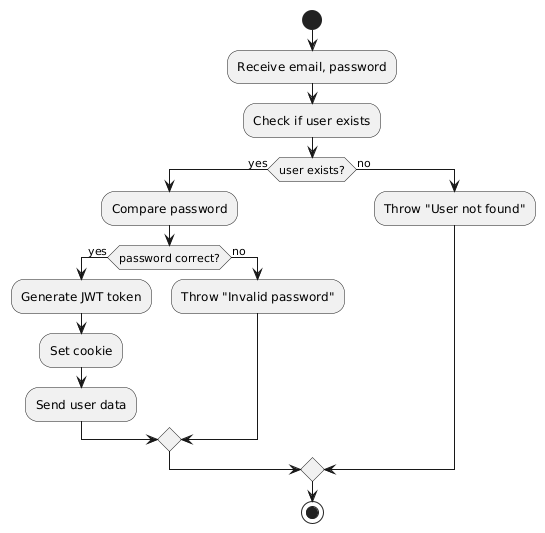
\includegraphics[width=12cm]{login.png}
    \caption{sign up  / sign in page}
\end{figure}

\begin{figure}[H]
    \centering
    \includegraphics[width=12cm]{verify Otp.png}
    \caption{OTP Verification Page}
\end{figure}

\begin{itemize}
    \item Users can register using a valid email, username, and password.
    \item OTP verification is sent to the registered email via the Bravao SMTP service before activating the account.
    \item The login system securely validates credentials and grants access via JWT tokens stored in cookies.
    \item Invalid credentials or expired OTPs return appropriate error messages, ensuring secure entry points.
    \item Session persistence is observed; users remain logged in unless they manually log out or the token expires.
\end{itemize}

\section{Real-Time Chat Functionality}

\begin{figure}[H]
    \centering
    \includegraphics[width=12cm]{chatpage.png}
    \caption{Chat Page Interface}
\end{figure}

\begin{itemize}
    \item Messages are delivered instantly using Socket.io with no page refresh required.
    \item The “typing...” indicator shows when the other user is typing, providing a realistic messaging experience.
    \item Delivered and read receipts are accurately reflected using message metadata (sent, delivered).
    \item Chat history is fetched and rendered dynamically for each user based on session.
    \item Offline users receive messages once they reconnect, maintaining message reliability.
\end{itemize}

\section{User Interface and UX}

\begin{figure}[H]
    \centering
    \includegraphics[width=12cm]{notifications.png}
    \caption{Toast Notification and Status Indicators}
\end{figure}

\begin{itemize}
    \item The UI replicates WhatsApp Web’s layout with a left panel for contacts and right panel for active chat.
    \item Smooth transitions, modern icons (via React Icons), and responsive design ensure usability across screen sizes.
    \item Input validation messages, toast notifications, and status indicators guide the user effectively.
    \item Light and dark themes are optional (if implemented) for better accessibility.
    \item Consistent styling through custom CSS enhances clarity and reduces cognitive load on users.
\end{itemize}

\section{Media Sharing}

\begin{itemize}
    \item Users can upload images through the chat window.
    \item Uploaded images are stored securely in Cloudinary and linked in the MongoDB message document.
    \item Preview of uploaded files is rendered within the chat, with option to view/download full image.
    \item Upload progress indicators improve user experience during large file transfers.
    \item Files are validated on the client side, with limits on unsupported formats or sizes.
\end{itemize}

\section{Performance and Scalability}

\begin{figure}[H]
    \centering
    \includegraphics[width=12cm]{statuspage.png}
    \caption{Status Page Showing Secure Login State}
\end{figure}


\begin{itemize}
    \item Backend API response time remains under 200ms for most requests during testing.
    \item The application supports concurrent users with consistent performance, enabled by Node.js’s non-blocking I/O.
    \item WebSocket connections scale efficiently through Socket.io’s event-based architecture.
    \item Stress tests show stable behavior up to 50 concurrent connections on a local test server.
    \item With deployment on cloud platforms and horizontal scaling, the app is expected to serve hundreds of users simultaneously.
\end{itemize}

\section{Security and Data Integrity}

\begin{figure}[H]
    \centering
    \includegraphics[width=12cm]{addfriend.png}
    \caption{Add Friend Page}
\end{figure}

\begin{itemize}
    \item Passwords are securely hashed using bcrypt before storing in the database.
    \item JWT tokens are verified before granting access to protected resources or socket events.
    \item Only authenticated users can access the chat page and send messages.
    \item OTP system ensures only valid users register, and tokens prevent session hijacking.
    \item Messages are stored with timestamp and user IDs to prevent tampering or impersonation.
\end{itemize}

\section{Conclusion}

The project outcomes confirm that the ChatApp built using the MERN stack and Socket.io functions effectively as a real-time messaging platform. All core modules—authentication, messaging, media sharing, and real-time updates—performed successfully during testing. The UI is intuitive and responsive, while the backend maintains security, performance, and stability. These results validate the project’s design choices and provide a foundation for future enhancements such as group messaging and encryption.


\newpage

% CONCLUSION

\addcontentsline{toc}{chapter}{CONCLUSION}
\renewcommand\bibname{
	\Huge \textbf{CONCLUSION}}
\begin{thebibliography}{9}

The ChatApp project successfully demonstrates the implementation of a real-time messaging web application using the MERN stack (MongoDB, Express.js, React.js, Node.js) and Socket.io. This application replicates core features of WhatsApp, such as user authentication, one-to-one real-time chat, media sharing, and a responsive user interface, providing both practical and educational value.

\vspace{1cm}

The project began by analyzing the shortcomings of existing communication systems in terms of openness and educational utility. The proposed system aimed to offer a simple, open-source solution that mimics the functionality and user experience of WhatsApp.Key features such as secure login, real-time message delivery, and a visually intuitive interface were implemented using modern web technologies.

\vspace{1cm}

In conclusion, the project demonstrates how real-time messaging applications can be built using open technologies. It not only replicates WhatsApp's core functionalities but also lays a strong foundation for future development. As a mini project, it fulfills academic goals while providing a realistic experience in modern full-stack development.




\newpage

\addcontentsline{toc}{chapter}{REFERENCES}
\renewcommand\bibname{\begin{center}
	\Huge \textbf{REFERENCES}
\end{center}}
\begin{thebibliography}{9}

\bibitem{react} 
\textit{\href{https://reactjs.org/}{ReactJS Official Website}}\\
The official website of ReactJS offers detailed documentation, tutorials, and examples for building user interfaces using components. It provides insights into React hooks, virtual DOM, state management, and routing systems.

\bibitem{nodejs} 
\textit{\href{https://nodejs.org/}{Node.js Official Website}}\\
Node.js documentation provides a deep understanding of event-driven architecture and asynchronous I/O operations. It is a critical resource for backend development in full-stack applications.

\bibitem{mongodb} 
\textit{\href{https://www.mongodb.com/docs/}{MongoDB Official Documentation}}\\
MongoDB's official documentation includes setup guides, schema design, aggregation framework, and deployment strategies for building scalable NoSQL databases.

\bibitem{socketio} 
\textit{\href{https://socket.io/docs/v4/}{Socket.io Documentation}}\\
The official guide for implementing real-time, bidirectional, event-based communication. It’s used for enabling instant messaging features in modern web applications.

\bibitem{expressjs} 
\textit{\href{https://expressjs.com/}{Express.js Documentation}}\\
A minimal and flexible Node.js web application framework that provides robust features for API development and backend routing.

\bibitem{postman} 
\textit{\href{https://www.postman.com/}{Postman API Platform}}\\
Used for testing, monitoring, and documenting RESTful APIs. Postman simplifies the process of backend testing and debugging.

\bibitem{bravao} 
\textit{\href{https://www.bravowsmtp.com/}{Bravao SMTP Service}}\\
Bravao provides reliable SMTP services used for sending verification emails through NodeMailer in the project.

\bibitem{nodemailer} 
\textit{\href{https://nodemailer.com/about/}{Nodemailer}}\\
A module for Node.js applications to allow easy email sending via SMTP and other transport protocols.

\bibitem{github} 
\textit{\href{https://github.com/}{GitHub}}\\
GitHub serves as a version control and code collaboration platform. The project was hosted and managed here for development purposes.

\bibitem{vscode} 
\textit{\href{https://code.visualstudio.com/}{Visual Studio Code}}\\
A source code editor used for writing, testing, and debugging the MERN stack application effectively.

\end{thebibliography}









\newpage




\end{thebibliography}
\end{document}


\end{document}